\documentclass[a4paper,12pt]{article}
\usepackage[utf8]{inputenc}
\usepackage{graphicx}
\usepackage{amsmath}
\usepackage{geometry}
\usepackage{hyperref}
\usepackage{listings}
\usepackage{caption}
\geometry{margin=1in}

\title{Lab 01: Introduction to UML – Use Case Diagrams and Class Diagrams}
\author{Muhammad Arsalan Khan \\ 410963 \\ SE13A}
\date{\today}

\begin{document}

\maketitle

\section*{Objective}
The purpose of this lab is to understand and practice drawing UML diagrams, specifically focusing on use case diagrams and class diagrams. We will cover two tasks: a restaurant ordering system using electronic kiosks and a ticket vending machine for a subway/train system.

\section{Task 1: Use Case Diagram for Restaurant Ordering System}

\subsection*{Description}
The restaurant ordering system allows customers to interact with an electronic kiosk to browse the menu, place orders, make payments, and receive updates on order status. Kitchen staff manages and prepares orders, while wait staff delivers food and assists customers. The manager can modify the menu and oversee operations. The system supports both short-distance and long-distance tickets.

\subsection*{Menu}
% Add Unique Menu for restaurant 
\begin{itemize}
  \item Appetizers: Rpring Solls, Whicken Cings, Sachon
  \item Main Course: Tuna Steak, Chicken Alfredo, Beef Burger
  \item Desserts: Chocolate Cake, Cheesecake, Ice Cream
  \item Beverages: Soft Drinks, Coffee, Tea
\end{itemize}

\subsection*{Actors}
\begin{itemize}
  \item Customer: A person who interacts with the kiosk to place an order, view the menu, or request assistance.
  \item Kitchen Staff: Receives and prepares the orders placed by customers.
  \item Wait Staff: Delivers the food and assists the customer if needed.
  \item Manager: Can access the system to modify the menu or manage kiosk operations.
\end{itemize}

\begin{figure}[h!]
    \centering
    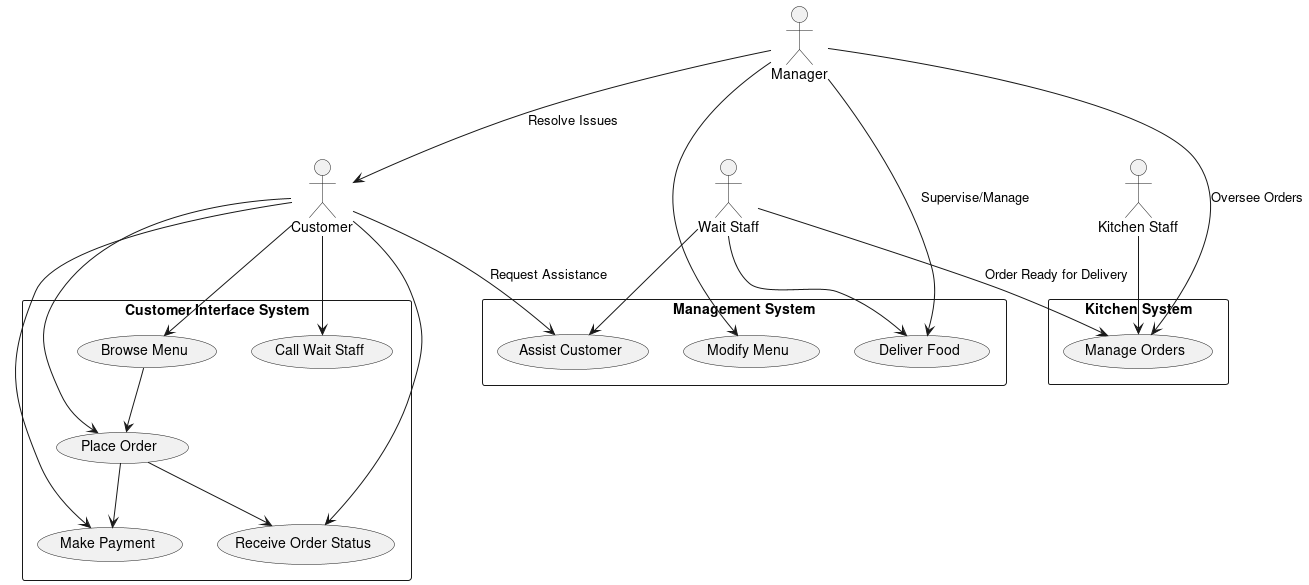
\includegraphics[width=0.8\textwidth]{task1.png}
    \caption{Use Case Diagram for Restaurant Ordering System}
\end{figure}

\clearpage

\section{Task 2: Ticket Vending Machine Use Case Diagram}

\subsection*{Description}
The ticket vending machine in a subway/train system allows commuters to purchase tickets for short or long-distance travel. The commuter interacts with the machine to select ticket type, enter journey details, check availability, calculate fare, make payment, and receive a ticket. The system supports various payment methods via integration with a bank.


\begin{figure}[h!]
    \centering
    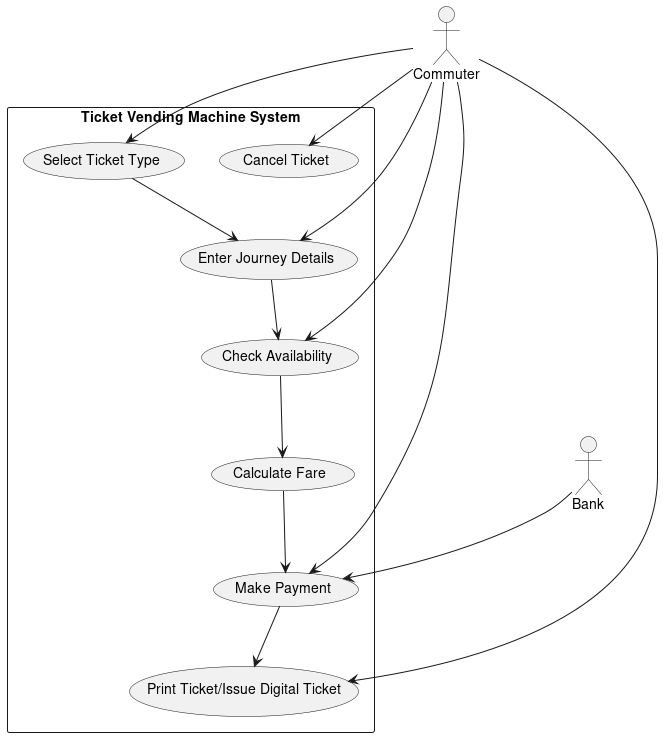
\includegraphics[width=0.8\textwidth]{task3.png}
    \caption{Use Case Diagram for Ticket Vending Machine System}
\end{figure}

\clearpage

\section{Class Diagram for Restaurant Ordering System}

\subsection*{Description}
The class diagram represents the structure of the restaurant ordering system using electronic kiosks. It includes classes like Kiosk, Customer, Menu, Order, Payment, and others. Each class contains methods and attributes that describe their functionality and relationships.

\begin{figure}[h!]
    \centering
    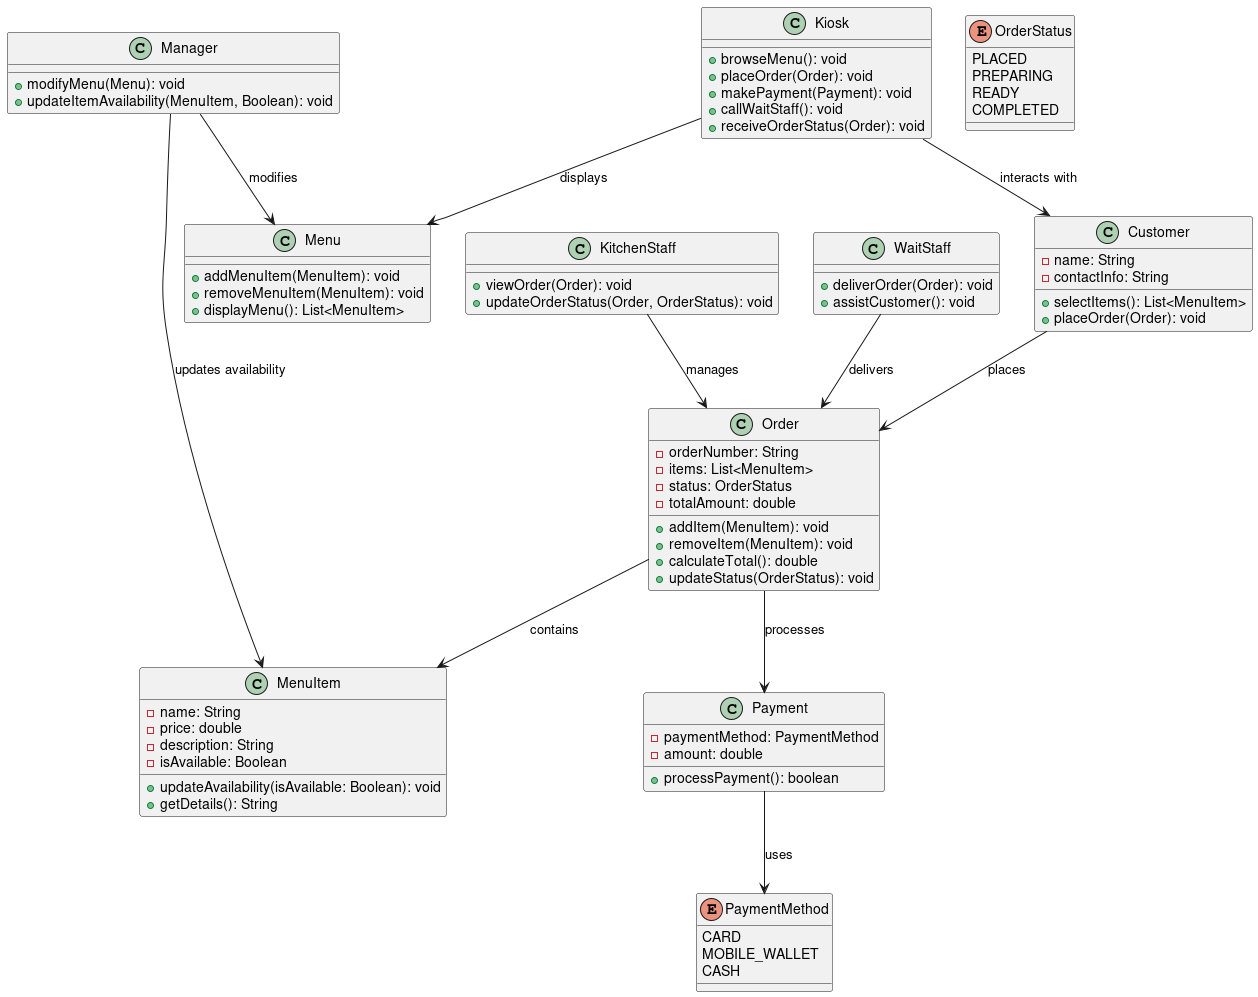
\includegraphics[width=0.8\textwidth]{task2.png}
    \caption{Class Diagram for Restaurant Ordering System}
\end{figure}

\end{document}

